\chapter{Résultats}
\section{Modes}
\label{resModes}

Pour mémoire, voici les résultats de différents modes obtenus avec freefem++.\\

\begin{figure}[H]
\makebox[\textwidth][c]{
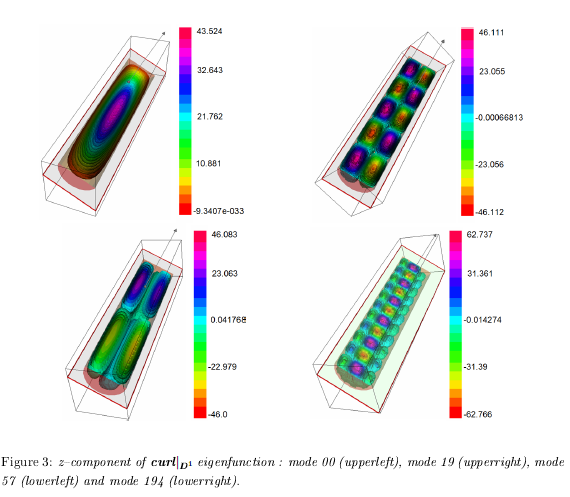
\includegraphics[scale=1]{Exemple_de_modes}}
\end{figure}

On peut voir les mêmes modes obtenus avec Feel++ dans la figure \ref{modes}.\\

\begin{figure}[H]
	\makebox[\textwidth][c]{
		\subfloat[mode00]{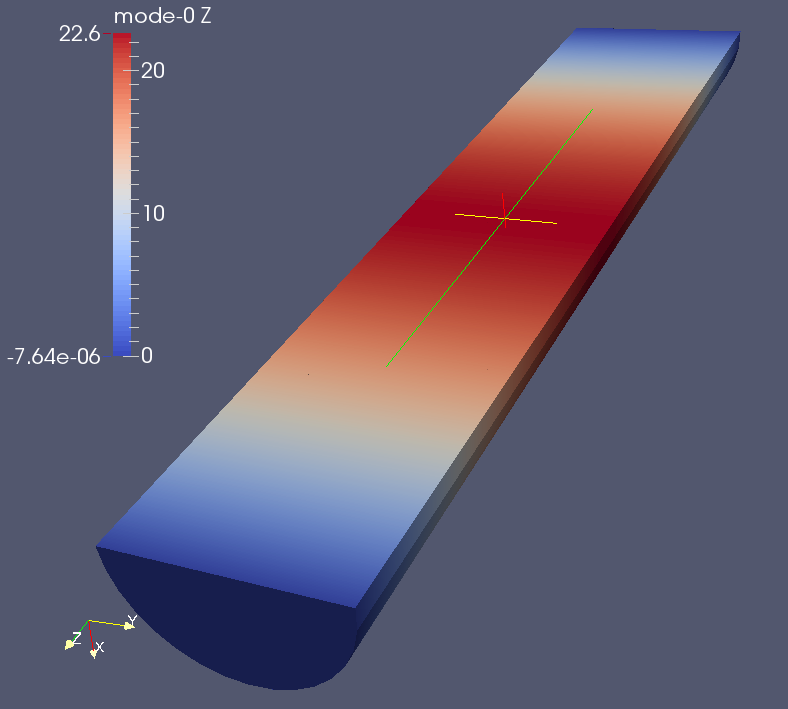
\includegraphics[scale=0.3]{mode00}}\ 
		\subfloat[mode19]{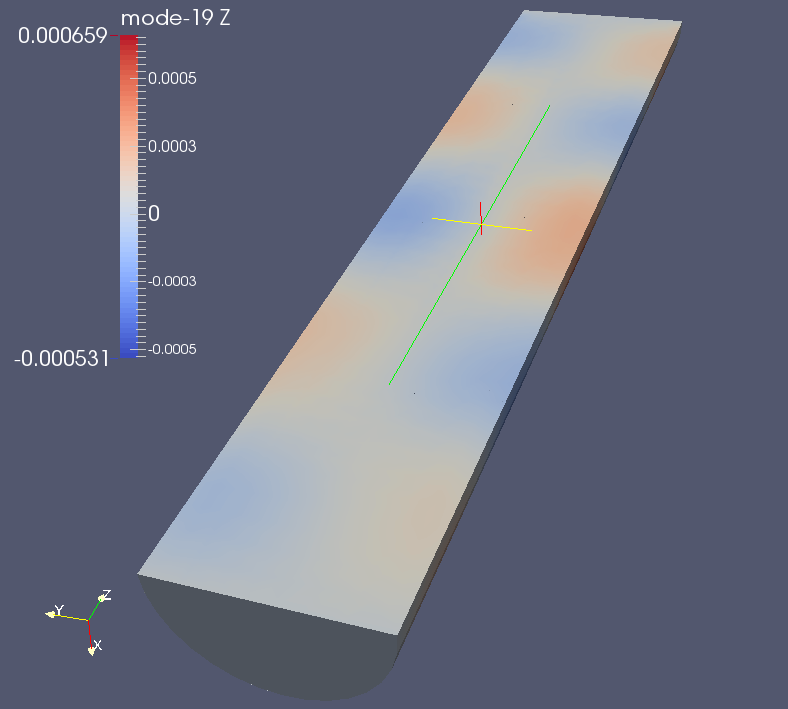
\includegraphics[scale=0.3]{mode19}}
	}\\
	\makebox[\textwidth][c]{
		\subfloat[mode57]{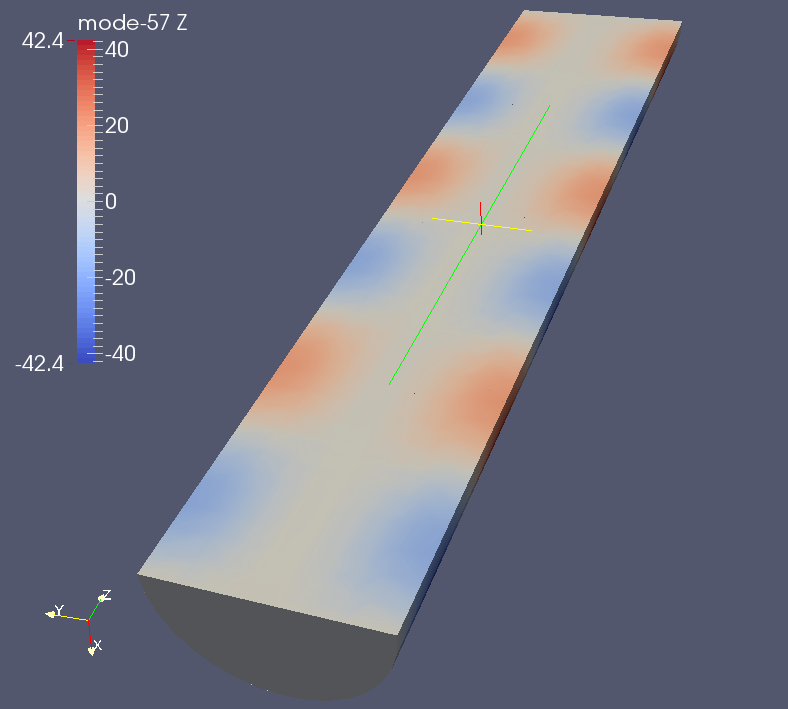
\includegraphics[scale=0.3]{mode57}}\ 
		\subfloat[mode194]{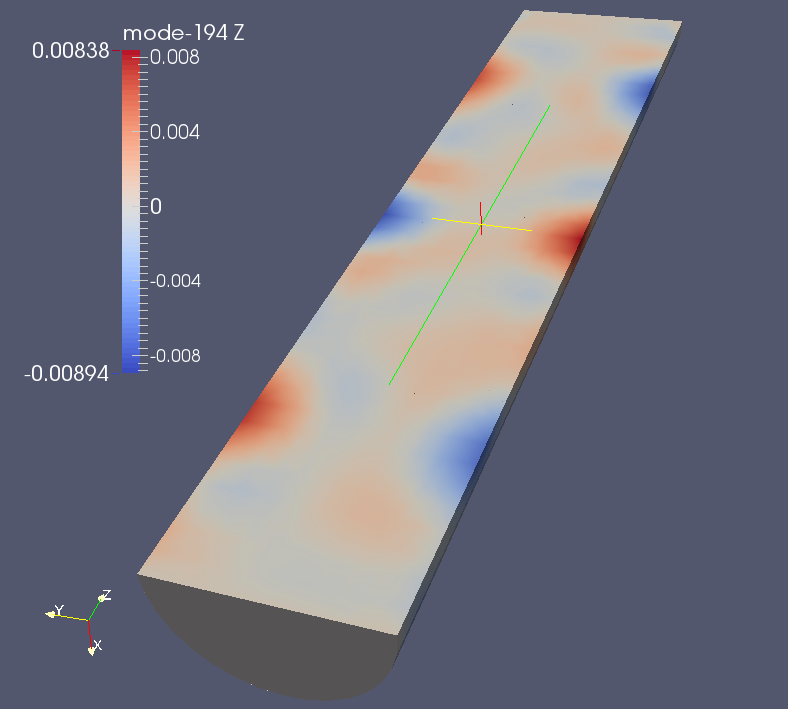
\includegraphics[scale=0.3]{mode194}}
	}
	\caption{composant z des fonctions propres}
	\label{modes}
\end{figure}

\iffalse

\section{Temps de calcul}

Les résultats précédents ont été obtenus sur 10 processeurs avec 200 valeurs propres et 300 valeurs propres convergées en 5536.05 sec, soit environ 1h30.\\

Faute d'installation de freefem++ sur le serveur de l'Irma, je n'ai pas pu effectuer de comparisons directe, mais j'ai lancé plusieurs fois l'application pour comparer le temps de calcul avec un même nombre de processeurs pour différents nombre de modes. Les résultats sont présentés dans la figure \ref{temps_proc}.\\

\begin{figure}[H]
\makebox[\textwidth][c]{
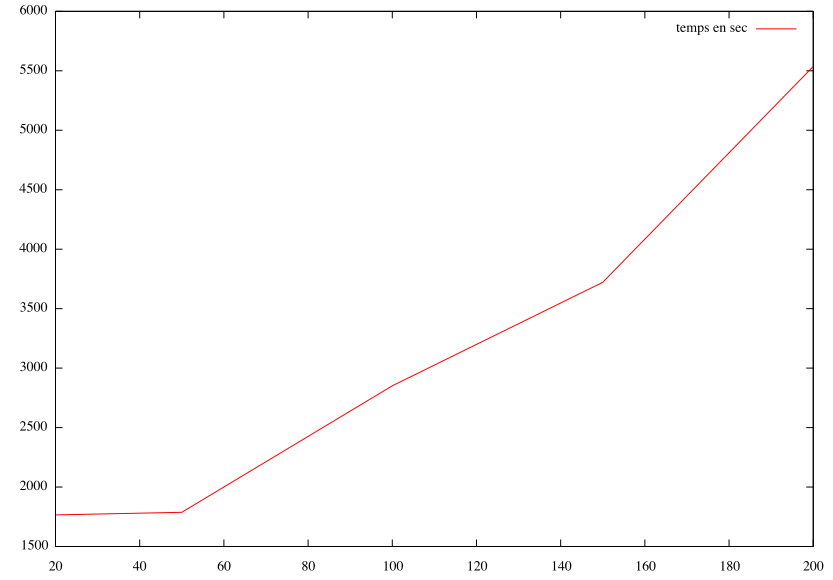
\includegraphics[scale=0.55]{temps_mode}}
\caption{Temps de calcul pour 10 processeurs avec 20, 50, 100, 150 et 200 modes}
\label{temps_proc}
\end{figure}

J'ai ensuite essayé de calculer le même nombre de modes avec un nombre différent de processeurs. Cette fois-ci, les résultats sont plutôt étranges. En effet, moins il y a de processeurs, plus le calcul est rapide, comme le montre la figure \ref{temps_mode}.

\begin{figure}[H]
\makebox[\textwidth][c]{
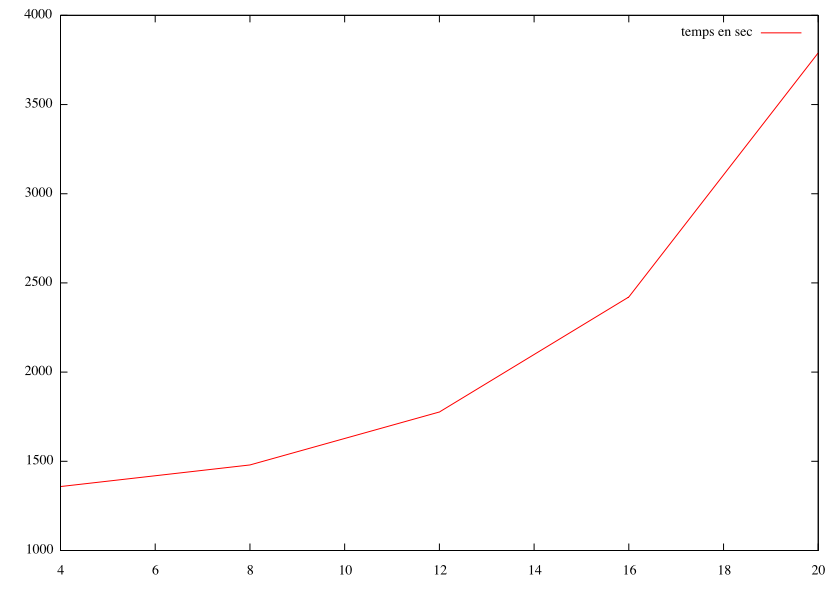
\includegraphics[scale=0.55]{temps_proc}}
\caption{Temps de calcul pour 50 modes avec 4, 8, 12, 16 et 20 processeurs}
\label{temps_mode}
\end{figure}

\fi

\section{Relèvement}

Dans la figure \ref{az}, on peut observer la composante en $z$ de $\mathbf{a}$ dans le cylindre, lorsque $\alpha_1=0$. Ce résultat a été obtenu avec le programme du chapitre \ref{gradh1}. 

\begin{figure}[H]
\makebox[\textwidth][c]{
  \subfloat{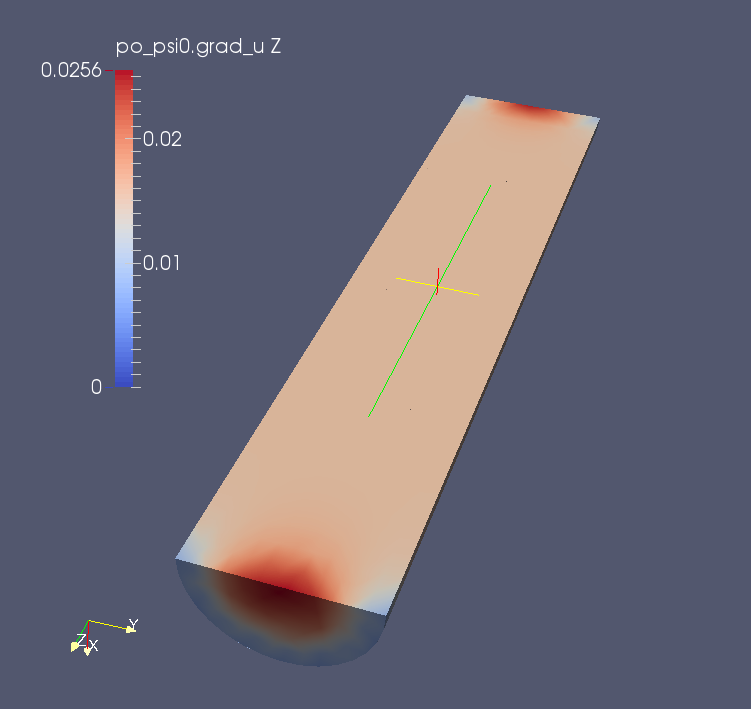
\includegraphics[scale=0.3]{az}}\ 
  \subfloat{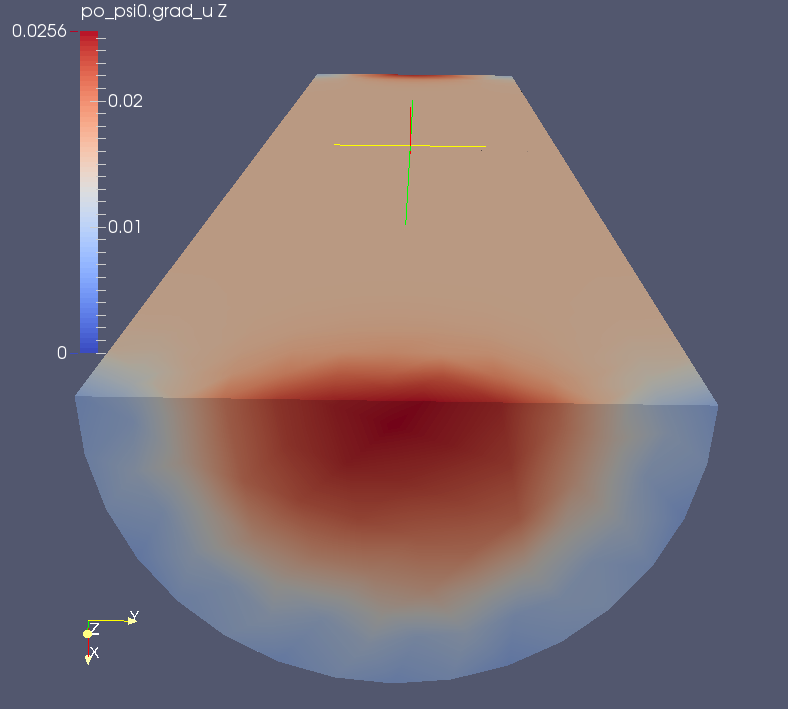
\includegraphics[scale=0.3]{az1}}
}
\caption{$\mathbf{a}=\grad\psi^0\in H(div)$}
\label{az}
\end{figure}
